\let\negmedspace\undefined
\let\negthickspace\undefined
\documentclass[journal]{IEEEtran}
\usepackage[a5paper, margin=10mm, onecolumn]{geometry}
%\usepackage{lmodern} % Ensure lmodern is loaded for pdflatex
\usepackage{tfrupee} % Include tfrupee package

\setlength{\headheight}{1cm} % Set the height of the header box
\setlength{\headsep}{0mm}     % Set the distance between the header box and the top of the text

\usepackage{gvv-book}
\usepackage{gvv}
\usepackage{cite}
\usepackage{amsmath,amssymb,amsfonts,amsthm}
\usepackage{algorithmic}
\usepackage{graphicx}
\usepackage{textcomp}
\usepackage{xcolor}
\usepackage{txfonts}
\usepackage{listings}
\usepackage{enumitem}
\usepackage{mathtools}
\usepackage{gensymb}
\usepackage{comment}
\usepackage[breaklinks=true]{hyperref}
\usepackage{tkz-euclide} 
\usepackage{listings}
% \usepackage{gvv}                                        
\def\inputGnumericTable{}                                 
\usepackage[latin1]{inputenc}                                
\usepackage{color}                                            
\usepackage{array}                                            
\usepackage{longtable}                                       
\usepackage{calc}                                             
\usepackage{multirow}                                         
\usepackage{hhline}                                           
\usepackage{ifthen}                                           
\usepackage{lscape}
\begin{document}

\bibliographystyle{IEEEtran}
\vspace{3cm}

\title{1.7.7}
\author{EE24BTECH11026 - G Srihaas}
% \maketitle
% \newpage
% \bigskip
{\let\newpage\relax\maketitle}

\renewcommand{\thefigure}{\theenumi}
\renewcommand{\thetable}{\theenumi}
\setlength{\intextsep}{10pt} % Space between text and floats


\numberwithin{equation}{enumi}
\numberwithin{figure}{enumi}
\renewcommand{\thetable}{\theenumi}

\textbf{QUESTION} \\
For what value of P  the points $\brak{2,1}$, $\brak{P,-1}$ and $\brak{-1,3}$ are collinear. \hfill\brak{10,2019}.\\
\solution
 \begin{center}
	\begin{tabular}{|c|c|c|}
    \hline
    \textbf{Variable name} & \textbf{Description} & \textbf{Formula}\\ 
    \hline
		A  & The point in 2-D plane with coordinates & $\myvec{2\\ 1}$ \\
    \hline 
		B  & The point with unknown coordinate  & $\myvec{P \\ -1}$ \\
    \hline
		C  & The point in 2-D plane with coordinates & $\myvec{-1\\3}$ \\
    \hline   
    \end{tabular}
\end{center}


Three points $\vec{A}$, $\vec{B}$ and $\vec{C}$ are said to be collinear if $$\emph{rank}\myvec{\vec{C}-\vec{B} & \vec{B} - \vec{A}} = 1 $$ \\
\begin{align}
\myvec{ -1-P & P-2 \\
         4 & -2 } 
\xleftrightarrow[]{R_1 \rightarrow {R_1/(-P-1)}}\quad
\end{align}
\begin{align}
\myvec{ 1 & \frac{2-P}{P+1} \\
         4 & -2 } 
\xleftrightarrow[]{R_2 \rightarrow {R_2-4R-1}}\quad
\end{align}
\begin{align}
\myvec{ 1 & \frac{2-P}{P+1} \\
         0 & \frac{2P-10}{P+1} } 
\end{align}
For the rank of the matrix to be one, $2P-10=0$.\\
$P-5=0$.\\
$P=5$.


\begin{figure}[ht]
	\centering
	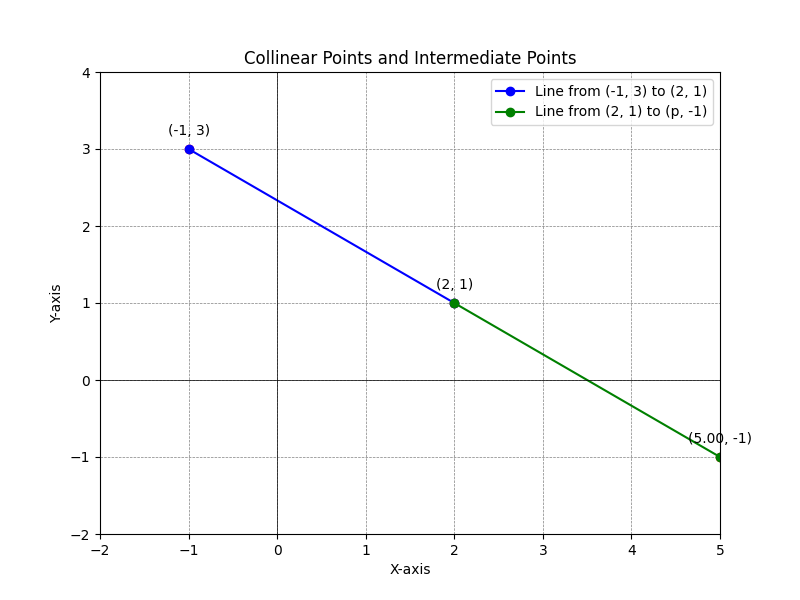
\includegraphics[width=0.8\textwidth]{figs/fig.png}
	\caption{A plot of the given question.}
	\label{fig:Plot1}
\end{figure}

	


\end{document}
